\documentclass[a4paper, titlepage, oneside]{article}

\usepackage[utf8]{inputenc}
\usepackage[australian]{babel}
\usepackage[vmargin = 2 cm, hmargin = 2 cm]{geometry}
\usepackage{multicol}
\usepackage{csquotes}
\usepackage{amsmath, amssymb}
\usepackage[cdot, amssymb]{SIunits}
\usepackage{graphicx, float}
\usepackage[outdir = ./build/]{epstopdf}
\usepackage{aasmacros}
\usepackage[backend = biber, style = authoryear, alldates = iso8601]{biblatex}
\usepackage[colorlinks = true, pdfpagemode = UseNone, pdfstartview = FitH]{hyperref}

% \usepackage{listings}
% \usepackage{xcolor}
% \usepackage{csvsimple}

% inputenc  : UTF-8 support for non-ASCII characters
% babel     : set language, for packages that need it
% geometry  : page margins
% multicol  : multiple columns
% csquotes  : context-sensitive quotes
% amsmath   : maths
% amssymb   : maths (\square redefined by SIunits)
% SIunits   : management of SI units; encourage using \unit{value}{units} command whenever possible
% graphicx  : \includegraphic
% float     : float graphics
% epstopdf  : use of eps files in document
% aasmacros : CUSTOM - assumes user has aasmacros.sty installed
% biblatex  : bibliography
% hyperref  : in-document links

% listings  : import external code
% xcolor    : more powerful engine for colour formatting
% csvsimple : import csv tables

% biblatex setup
\renewcommand{\nameyeardelim}{\addcomma\addspace} % Change delimiter for in-line citations to include a comma
\addbibresource{group-report.bib}

% hyperref setup
% \hypersetup{allcolors = blue} % Override all link colours
% \hypersetup{hidelinks} % Links will be shown with neither boxes nor colours

% Custom macros
\newcommand{\elem}[2]{\textsuperscript{#1}{#2}}
\newcommand{\molec}[2]{\ensuremath{\text{#1}_{#2}}}
\newcommand{\ion}[2]{#1~\smallcaps{#2}} % Must use lowercase Roman numerals eg, \ion{H}{ii}
\newcommand{\e}[1]{\ensuremath{\times 10^{#1}}}
\newcommand{\smass}{\mathrm{M_\odot}}
\newcommand{\parsec}{\mathrm{pc}}

% Document
\begin{document}
\title{\textbf{Searching for molecular gas towards TeV gamma-ray sources: Analysing 3D data cubes of the molecular gas tracer carbon monoxide with images from the HESS gamma-ray telescopes}}
\author{R.~M. Harvey \and K.~T. Leaver \and H.~D. Poulter}
\date{13 October 2014} %Leave blank to print no date, or you can type in the desired date
\maketitle

\setcounter{page}{1}
\pagenumbering{roman}
\numberwithin{equation}{section}

\tableofcontents

\clearpage
\setcounter{page}{1}
\pagenumbering{arabic}

\begin{center}
  {\large \textbf{Searching for molecular gas towards TeV gamma-ray sources: Analysing 3D data cubes of the molecular gas tracer carbon monoxide with images from the HESS gamma-ray telescopes}}

  \vspace{1.5em}

  R.~M. Harvey\footnote{Molecular clouds and cosmic ray interactions} \quad K.~T. Leaver\footnote{\elem{12}{CO} and \elem{13}{CO} as tracers} \quad H.~D. Poulter\footnote{Galactic rotation, Noise anaylsis, HESS J1632-479}
\end{center}

\vspace{1.5em}

\begin{minipage}{0.93\textwidth}
  \begin{abstract}
  This report is about finding the TeV sources and molecular clouds associated with such sources. It beings with a brief overview of the types of physical and astronomical concepts behind the science that has been used in writing up the report and making the conclusions.
  \end{abstract}
\end{minipage}

\vspace{1em}

\begin{multicols}{2}
\section{Introduction}
\paragraph{}
TeV gamma-ray sources are among the most energetic sources known to exist in the [galaxy/universe/multiverse]. They are theorised to arise from cosmic ray sources (CITE-REF)

\section{Theory}
\paragraph{}
Theory stuff goes in here, including but not limited to:
\begin{itemize}
  \item Cosmic ray sources
  \item Large molecular clouds, and their interactions with CRs
  \item CO \& \elem{13}{CO} as tracers
  \item Telescope information/general data stuff?
  \item Galactic rotation/Doppler shift in Mopra data
\end{itemize}
Fun! These titles are all outdated! We won't use these!

\subsection{Featured telescopes}
\paragraph{}

The HESS Cherenkov Telescope system is a telescope array that detects high energy gamma rays (\(\sim\)\(3\e{10}\) to \unit{10^{14}}{\electronvolt}). We received data showing the detected intensity for the three gamma ray sources as single frame fits files, the value associated with each pixel representing the number of gamma ray counts in the energy band of the observations. This data allowed the location, intensity and extent of the three sources to be determined. The primary data used to analyse the potential source candidates for the gamma rays was gathered by the Mopra Radio Telescope. Data for both \elem{13}{C}O and \elem{12}{C}O (see section~\ref{sec:co}) was used in data cube format, where the doppler shift of the emission lines of the CO has been convcerted to relative velocity. The data cube contains several thousand frames that span \(\sim\)\unit{1000}{\kilo\meter\cdot\reciprocal\second} and are used to represent the distance to the source of the emissions.

\subsection{Cosmic ray sources}
\paragraph{}
Whoa! Need a whole lot of words right here very quickly. Okay let's see um.

First, you must spread a thick layer of peanut butter onto the white part of a slice of bread. You can only spread the peanut butter on the white part, and the white part only. You may only spread peanut butter on one side. Spreading peanut butter on both sides will provide an inferior sandwich. Next, you must spread a thick layer of jam onto the white part of a slice of bread. You can only spread the jam on the white part, and the white part only. You may only spread jam on one side. Spreading jam on both sides will provide an inferior sandwich. You cannot spread jam onto the same slice of bread onto which you have spread peanut butter. Also, you cannot spread peanut butter or jam onto more than one slice of bread, as this will provide an undesired excess of either ingredient. Additionally, only peanut butter and jam can be spread onto these slices of bread; no other ingredient will suffice, and no substitute can be used in a sandwich that is to be legitimately recognized as a peanut butter and jam sandwich. Likewise, only bread may be the substance upon which the peanut butter and jam are spread, as anything else does not fit the standards of a peanut butter and jam sandwich; if the peanut butter and jam are spread onto a culinary medium that isn’t bread, the meal at hand simply is not a peanut butter and jam sandwich. Once you have accomplished spreading a thin layer of peanut butter onto the white of one side of one slice of bread, and likewise has been accomplished using raspberry jam on a separate slice of bread, you must match the slices of bread up to each other, forming a peanut butter and jam sandwich. In this scenario, the peanut butter-covered face of bread must be facing the jam-covered face of the second slice of bread so that the peanut butter surface touched the surface of the jam. The surface of the peanut butter is not allowed to touch a jam-less substance of bread, resulting in the jam facing outwards, and likewise applies to the jam. If a substance is found facing on the outside of the sandwich, the product will not be accepted as a peanut butter and jam sandwich. The side with peanut butter and the side with jam on it must match up and stick together to form one solid sandwich. When the eater picks up the sandwich, he or she must hold both pieces of bread at the same time, or else one slice will fall off, and eating only one slice of bread will not be recognized as the same or even similar to eating a peanut butter and jam sandwich.

\subsection{Galactic rotation}
\label{sec:gal-rot}
\paragraph{}
The Mopra data featured heavily in this report \parencite{Burton:2013} derives its usefulness from the effect that galactic rotation has on objects along the line of sight across the Milky Way. Fig.~\ref{fig:gal-rot} shows how for a simplified model of the Milky Way with constant radial velocity, looking along a line of sight, in this particular instance one corresponding to a galactic latitude of \(l=337\), leads to a velocity gradient and a measurable Doppler shift. In order to find distances from the sun using the Mopra data, it is necessary to consider the component of velocity parallel to the line of sight. As derived in Appendix~\ref{app:doppler}, the velocity of an object along the line of sight with galactic latitude \(l\) is given by
\begin{equation}
  v_{los}(d)=\frac{v(R)R_0\sin{l}}{\sqrt{d^2-2R_0d\cos{l}+R_0^2}}-v(R_0)\sin{l}\;\,,
\end{equation}
where the distance from the sun to the galactic centre (GC) is \(R_0\), and distance from the sun to the object of interest is \(d\). This equation holds for a galaxy with variable rotation \(v(R)\) dependent on radial distance \(R\) from the GC. For the sake of simplicity in this report, this expression is taken to be a constant \(v(R)=\unit{220}{\kilo\metre\usk\reciprocal\second}\), as suggested by \textcite{Kerr:1986}. They also suggest a value for the distance from the GC to be \(R_0=\unit{8.5}{\kilo\parsec}\).

\begin{figure}[H]
  \centering
  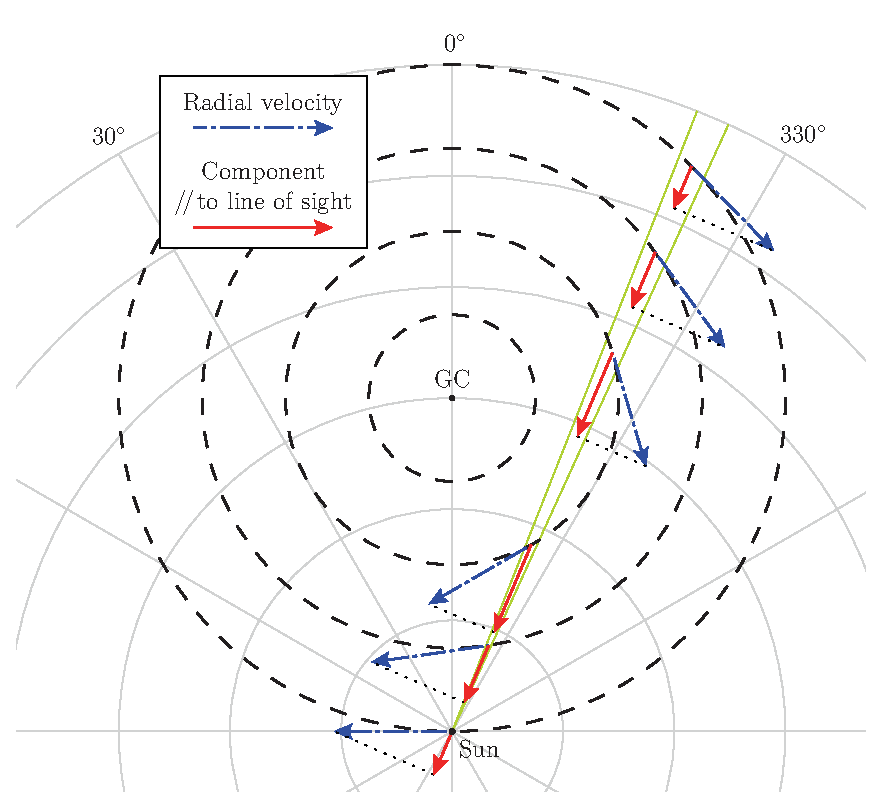
\includegraphics[width = \columnwidth]{figures/galactic-rotation}
  \caption{Galactic rotation showing Doppler shifts}
  \label{fig:gal-rot}
\end{figure}

\subsection{Molecular clouds}
\subsubsection{Composition and structure}
\paragraph{}
The average density of the interstellar medium (ISM) is quite low, however the reaches of space are littered with so-called molecular clouds -- areas with gas and dust density significantly higher, such that stars can form within the material. These clouds are predominantly composed of molecular hydrogen (\molec{H}{2}), which for reasons to be discussed in Section~\ref{sec:co} is relatively difficult to detect. However, the presence of carbon monoxide (CO) is significantly easier to determine, and astrophysicists presently believe it to be distributed among \molec{H}{2} in effectively equal quantities, making it an excellent tracer \parencite{Glover:2011}.

Gas and dust formations with a total mass between \(10^3\) and \unit{10^7}{\smass} are called giant molecular clouds (GMCs), and tend to be anywhere from 5 to 200 parsecs in diameter \parencite{Murray:2011}. `Diameter' is a term applied fairly loosely, as the form of a GMC is not guaranteed to be even remotely spherical. Indeed, the tenuous structural qualities of GMCs mean that they can also vary greatly in density, typically from around \(2\e{-20}\) to \unit{2\e{-18}}{\gram\usk\centi\metre\rpcubed}, corresponding to approximately \(10^4\) to \(10^6\) molecules per cubic centimetre \parencite{Ferriere:2001}.

\subsubsection{Interactions with cosmic rays}
\paragraph{}
Cosmic rays incident on GMCs can through a variety of mechanisms produce gamma rays, in our case often within TeV range and hence detectable by the HESS telescope. Bremsstrahlung radiation is motivated by Coulombic forces, and results from inbound cosmic rays being deflected by charged particles present in the interstellar gas, this change thus emitting gamma radiation. Inverse Compton scattering is motivated by conservation of momentum, and involves high-energy cosmic rays colliding with ``soft'' photons in the gas, exchanging momentum and in the process resulting in a more energetic photon with energies in TeV ranges \parencite{Ferriere:2001}. The synchrotron effect may also produce gamma rays, but is not included in this data set as HESS is not sensitive to such effects.

\subsubsection{Kinetic energy of expanding bubbles}
\label{sec:kinetic}
\paragraph{}
Powerful events in GMCs -- such as supernovae -- can push away all nearby gas, clearing out distinct ``bubble'' regions readily visible in images of gas distributions. In order to find the energy released by the event, we simply need find the kinetic energy of the gas which is now moving away, assuming it previously had negligible kinetic motion and almost all of the energy released by the event has been transferred to the surrounding gas.

The Mopra data cubes provide redshift speeds for each image slice, hence permitting us to find the relative speeds of two areas of gas, such as the two sides of an expanding bubble. For the full derivation please see Appendix~\ref{app:kinetic}, however the final result is replicated here:
\begin{equation}
  \label{eq:KE}
  \mathrm{KE} = \frac{\pi ^ 4}{6} {\left( \frac{\Delta l}{360} \right)}^3 \rho d^3 {(v_1 - v_2)}^2 \, \joule \, ,
\end{equation}
where \(\Delta l\) is the maximum angular width of the bubble in degrees, \(\rho\) is an estimate of the mass density in \(\kilo\gram\usk\centi\metre\rpcubed\) of the gas previously occupying that volume, \(d\) is the distance to the centre of the bubble in \(\centi\metre\), and \(v_1\) and \(v_2\) are the redshift speeds of the front and back of the bubble in \(\metre\usk\reciprocal\second\).

\subsection{Carbon monoxide as a tracer for molecular hydrogen}
\label{sec:co}
\paragraph{}
The majority of the hydrogen in the galaxy is in either atomic or molecular form. Atomic hydrogen can emit a photon because of the energy difference between the electron and proton having parallel and anti-parallel spins. This spin transition for the electron results in the emission of a photon with a wavelength of \unit{21}{\centi\metre}. Molecular hydrogen (\molec{H}{2}) has very weak emission lines due to its high symmetry, and at the extremely low molecular cloud temperatures of \(\sim\)\unit{10}{\kelvin}, molecular hydrogen is completely undetectable. Thankfully, carbon monoxide (CO) is asymmetric and occurs alongside \molec{H}{2} in a mostly uniform ratio throughout our galaxy \parencite{Neininger:1998}. The CO is hit by neighbouring molecules and gains energy in either rotational or vibrational stretching forms. These energy modes are quantised, and when the rotation or vibration drops an energy level a photon will be emitted. Because each isotopologue will have a different moment of inertia and therefore different energy levels, the frequency of the photon will depend on both the isotopologue and the energy levels between which the transition occurs. Because of this it is possible to look for specific isotopologues and specific energy transitions, which, knowing how they are distributed with \molec{H}{2}, allows the mapping of molecular clouds.

\section{Data analysis}
\paragraph{}
In this section, analytical techniques such as noise analysis, kinematic analysis and analysis of the Mopra CO data are outlined and discussed.

\subsection{Noise analysis}
\paragraph{}
A vital aspect of the analysis of data from HESS, Mopra, and other data sources involved estimating the level of background noise associated with each data set, and making judgements regarding the cut-off level where the data became valid signal. Fig.~\ref{fig:noise} shows a schematic idealisation of the histograms for the data sets used in the report. In order to plot accurate contours of gas clouds, and hence properly analyse them, the levels had to be set so that background counts were effectively removed. Each data set has already had a defined number of background counts subtracted from it, thus leading to the existence of points with negative numbers of counts. This in turn meant the formation of an associated background count roughly distributed as a Gaussian curve due to its random nature, as seen in Fig.~\ref{fig:noise}. In order to only plot contours on values considered to be signal, and correctly ignore the background noise, we considered the standard deviation \(\sigma\) of the background. As we expected the number of counts for the signal to be in the positive domain, we focused on the negative side of the histogram and used it to estimate the value of the standard deviation \(\sigma\) in the background noise, using the approximate ``bell curve'' present in the negative domain. In order to be more certain that only the signal was then considered, the value for \(\sigma\) was doubled, and this used as the lower contour limit. Thus, for the normally-distributed background noise, only 2.3\% of the noise would be included in the statistically-significant contour levels. This allowed further analyses on the sources to clearly identify the signal from the noise, and hence have much stronger accuracy.

\begin{figure}[H]
  \centering
  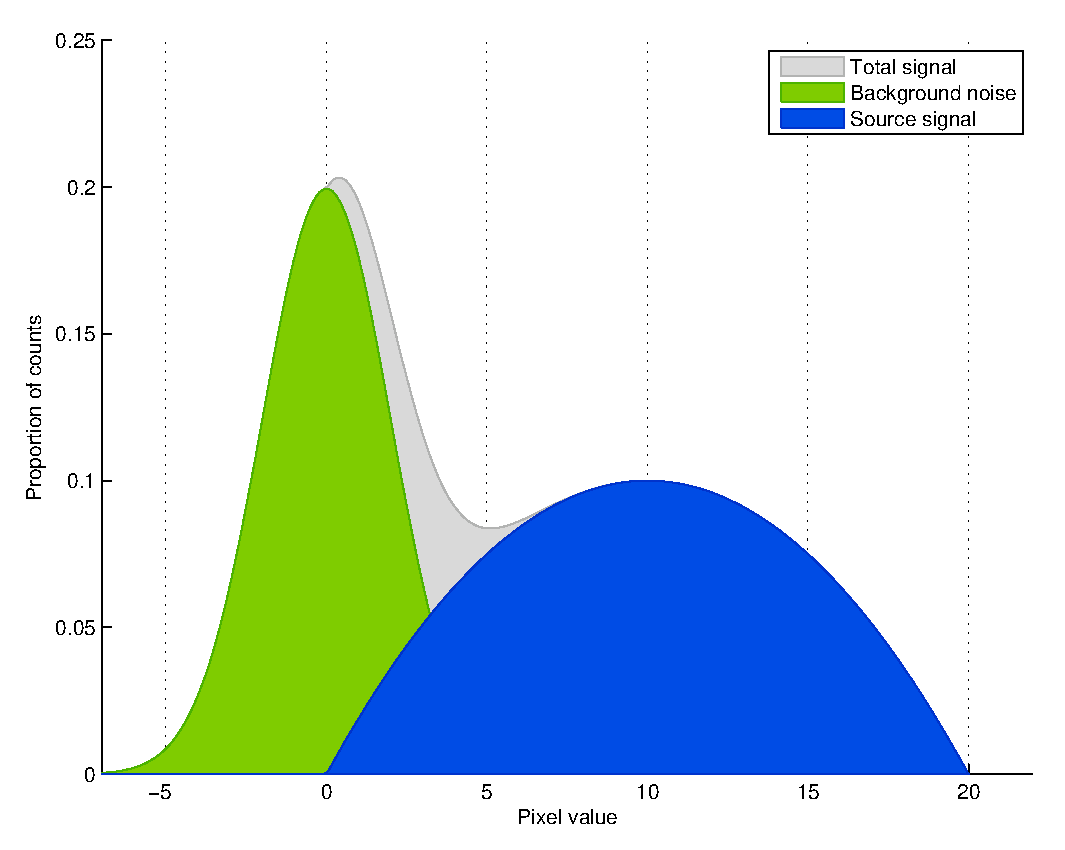
\includegraphics[width = \columnwidth]{figures/noise-analysis}
  \caption{Representative graph of the signal histogram}
  \label{fig:noise}
\end{figure}

\subsection{Kinematics}
\paragraph{}
Several gas clouds have formations highly suggestive of bubbles formed due to supernova explosions. Using the techniques outlined in Section~\ref{sec:kinetic}, we subsequently calculate the energies of those bubbles.

\subsubsection{IGR J16358-4726}

\begin{figure}[H]
  \centering
  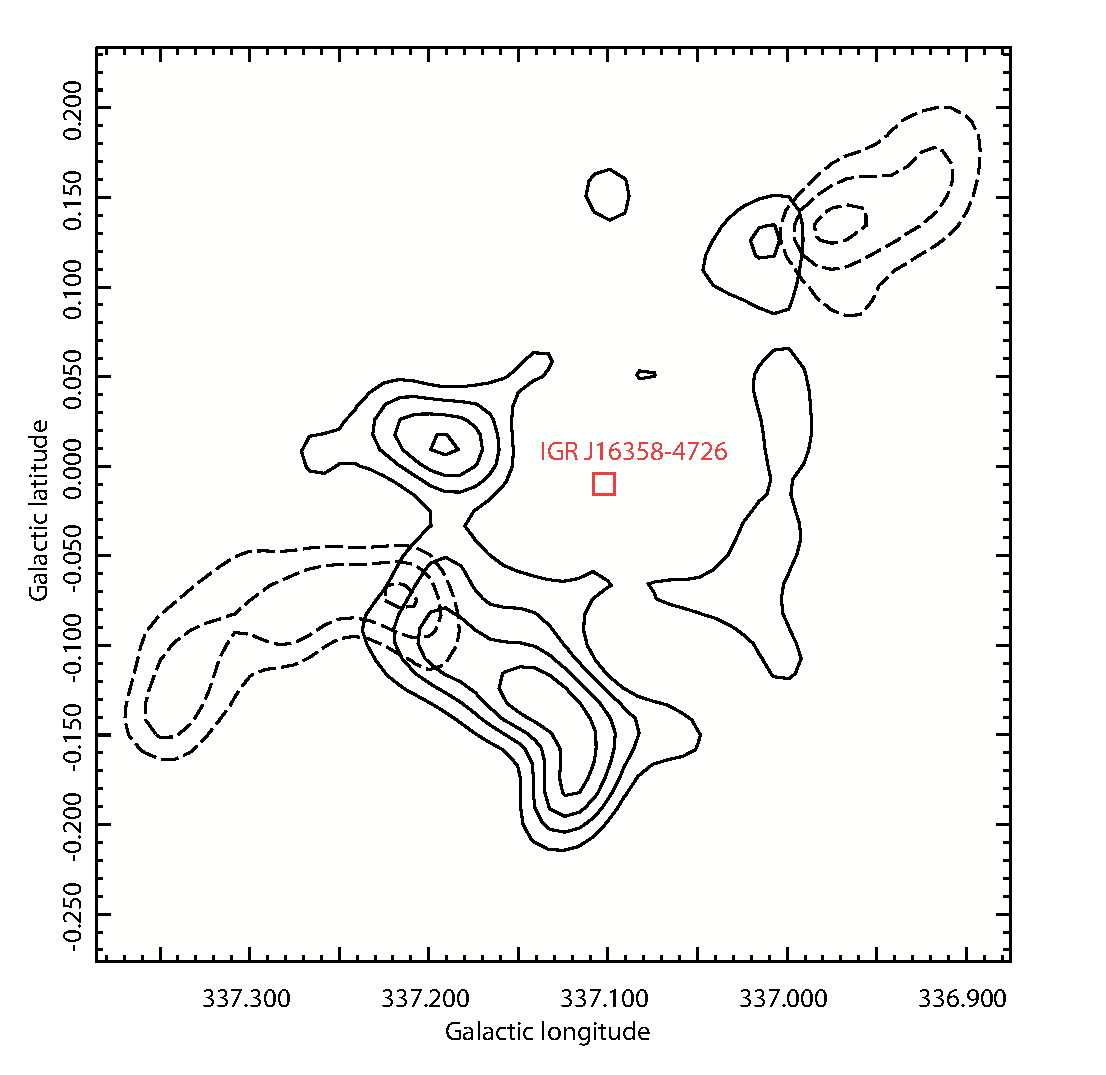
\includegraphics[width = \columnwidth]{figures/bubble34}
  \caption{Composite image of three frames best illustrating the bubble around IGR J16358-4726. The dashed contours are behind (lower left) and in front of (upper right) the solid central ones}
  \label{fig:bubble34}
\end{figure}

\paragraph{}
Fig.~\ref{fig:bubble34} shows the formation of a bubble around IGR J16358-4726, discussed further in Section~\ref{sec:hess34}. Applying Eq.~\ref{eq:d} for \(v(R) = v(R_0) = \unit{255.2\e{3}}{\metre\usk\reciprocal\second}\) and \(R_0 = \unit{8.34}{\kilo\parsec}\) \parencite{Reid:2014}, we find the central object to be either \(4.18\) or \unit{11.2}{\kilo\parsec} away, which agrees quite favourably with \textcite{Lutovinov:2005} who report near and far solutions for distance equal to \(5 - 6\) and \unit{12 - 13}{\kilo\parsec}, respectively. With these distances, we use Eq.~\ref{eq:KE} and assume an average uniform mass density \(\rho\) of \unit{2\e{-21 \mathrm{~to~} -23}}{\kilo\gram\usk\centi\metre\rpcubed} \parencite{Ferriere:2001} to find the bubble has kinetic energy \unit{9.34\e{42 \mathrm{~to~} 44}}{\joule} for the near solution and \unit{1.78\e{44 \mathrm{~to~} 46}}{\joule} for the far solution. Considering the average energy output of a supernova is of the order of \unit{10^{44}}{\joule} \parencite{Khokhlov:1993}, this is a very reasonable result.

\subsection{Carbon monoxide clouds}
\paragraph{}
Talk about the use of \elem{12}{C}O to find areas of bulk cloud structures, as well as \elem{13}{C}O to confirm these areas. It would also be worth a bit of discussion about where the CO clouds were located in general, I guess? What sorts of analysis did we really do on these clouds except finding areas of cloud line-up with various sources and/or other data sets. Could be worth putting a table in here like that on the docs just listing the observations made of the Mopra data. That sounds like an excellent idea, Harry. That'll go into an appendix for sure if I can't find out a way of making tables or figures in general span multiple columns. Look into using the \texttt{wrapfig} package maybe?

\section{Source candidates}
\paragraph{}
During the analysis of CO data from Mopra, as well as using the SIMBAD catalogue to plot high-energy sources, a few were set aside as possible candidates for the large gamma ray readings from HESS. In this section, the sources are discussed alongside their possible effect on the gamma-ray emission measured from HESS. Also, when are we going to chuck in various energy fluxes measured from the HESS sources, should those go in the part before the source candidates are listed for each source? I'll slap 'em in beforehand, yeah.

\subsection{HESS J1632-479}

\begin{figure}[H]
  \centering
  \frame{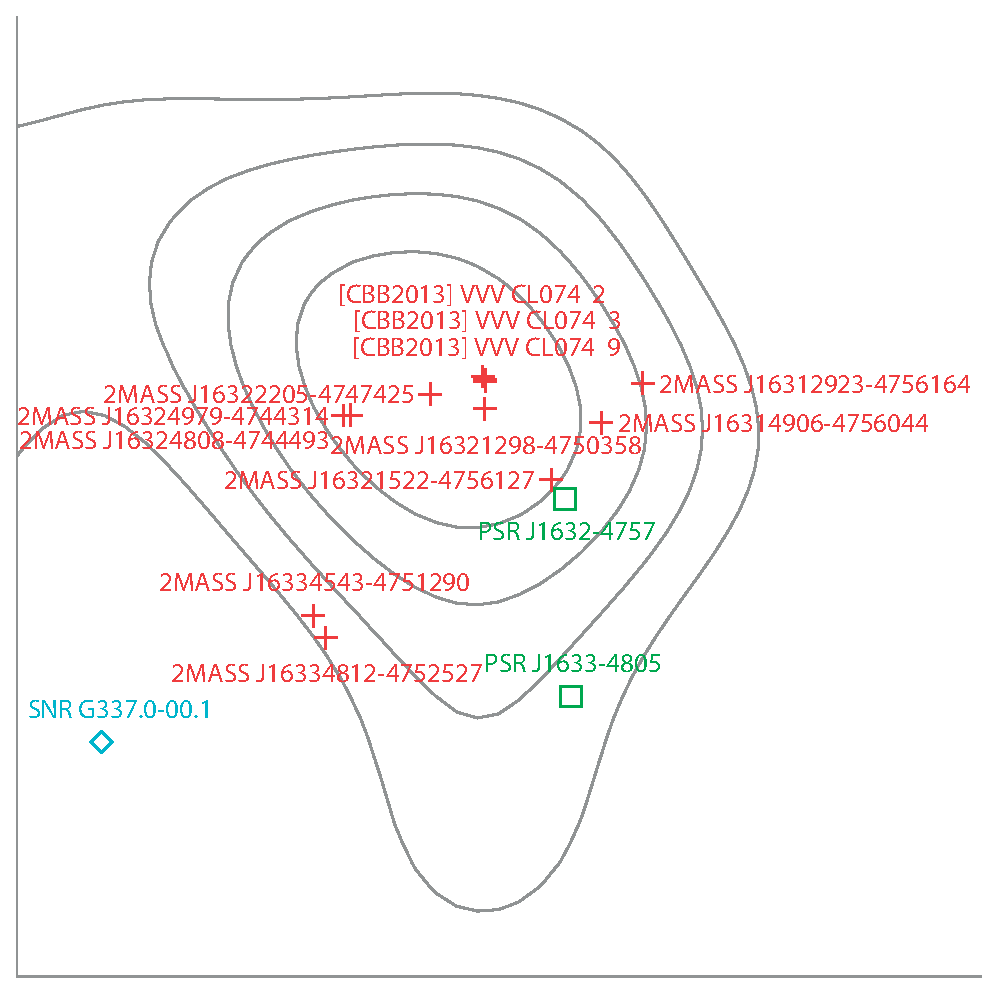
\includegraphics[width = \columnwidth]{figures/hess32}}
  \caption{Contour plot of HESS J1632-479 and surrounding objects of interest. Wolf-Rayet stars are shown as red crosses, supernova remnants as blue diamonds, and pulsars as green squares}
  \label{fig:hess32}
\end{figure}

\paragraph{}
Words about the gamma-ray source in question, and its possible source candidates goes here. The source candidates for this particular gamma-ray source include a Wolf-Rayet cluster, VVV CL074, and just Wolf-Rayet stars in general around the area. Probably not the pulsar or SNR, but I'll chuck in a discussion of the two anyway for more words and all that. Also, because anything's worth discussing when the possible source of these gamma-rays is so mysterious and spoopy.

\subsubsection{VVV CL074}
\paragraph{}
An object worthy of attention within this source is VVV CL074, a Wolf-Rayet open star cluster discovered by \textcite{Chene:2013}, which could be contributing to the total gamma ray emission. Worth noting is that in this open cluster one star in particular, VVV CL074 9, is given by \textcite{Chene:2013} to be at a distance of \unit{13.57}{\kilo\parsec}, while other stars in the cluster are within a distance of \unit{8}{\kilo\parsec}. This star in particular has a spectral class of WN7/O4–6If+ \parencite{Chene:2013}, giving it the possibility of it being either a Wolf-Rayet star (WR*) with prominent nitrogen lines in its spectra, or an O-type star with interesting spectral lines in it as well. \textcite{Chene:2013} also mentions that if it were an O-type star then it would only be at a distance of \(\unit{6.8}{\kilo\parsec}\). This suggests that it would be a very energetic Wolf-Rayet star, just at a very large distance so it would seem to be an O-type star.

Another intersting star is VVV CL074 3, with spectral classification WN8. What makes this star interesting lies in a paper by \textcite{Foellmi:2002}, which suggests that WR* of spectral type WN8 could be exotic Thorne-Zytkow objects. These objects are formed in binary systems where one companion star goes supernova, leaving a neutron star or blackhole behind. Due to the close proximity of the two stars, and the inherent `kick' given to the projenitor star after going supernovae, this could push the two objects into each other, undergoing a merge event where the companion star now contains the neutron star or blackhole, forcing it to expand. These sorts of objects could be a source of high energy particles or something of the ilk.

As a whole, the cluster has an estimated mass of over \unit{2500}{\smass} with a distance of \(\unit{6}{\kilo\parsec}\), meaning it is massive and also far away, so energy comes streaming out of it somehow. It's interesting enough to mention. Fig.~\ref{fig:hess32} shows where the bulk of these WR* are located in the cluster. It's a pretty small cluster in terms of angular size, but hey, things to do, people to meat.

\subsection{HESS J1634-472}
\label{sec:hess34}

\begin{figure}[H]
  \centering
  \frame{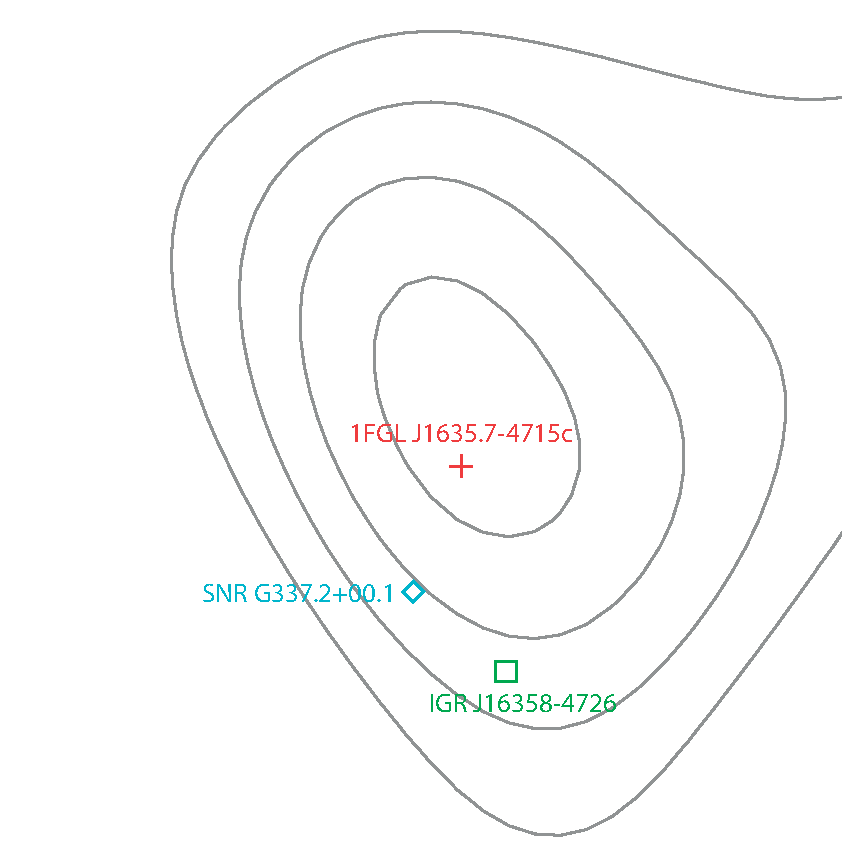
\includegraphics[width = \columnwidth]{figures/hess34}}
  \caption{Contour plot of HESS J1634-472 and surrounding objects of interest. Wolf-Rayet stars are shown as red crosses, supernova remnants as blue diamonds, and pulsars as green squares}
  \label{fig:hess34}
\end{figure}

\paragraph{}
There's an intersting pulsar IGR J16358-4726, but the two WR*s near that pulsar are pretty awful.

\subsubsection{IGR J16358-4726}
\paragraph{}
Also known as [KRL2007b] 194, this object is well within the bounds of HESS J1634-472 as depicted in Fig.~\ref{fig:hess34}. Originally discovered in 2003, before later being serendipitously observed by the Chandra X-Ray Observatory and classified as an x-ray transient \parencite{Patel:2004}. These are

Blah blah it has been proposed something something one of only a handful (at this time) of symbiotic x-ray binaries (SyXBs) -- a new subclass of low-mass x-ray binary system \parencite{Nespoli:2010}. SyXBs feature a compact object such as a neutron star orbiting and accreting matter from an M-type red giant star,

The kinematic analysis of the gas bubble around this pulsar gives a figure of \_\_\_\_. Reece, list your kinematic analysis in here damnit, or the results of that from the analysis.

\subsubsection{Wolf-Rayet stars}
\paragraph{}
2MASS J16345746-4704129

\subsection{HESS J1640-465}

\begin{figure}[H]
  \centering
  \frame{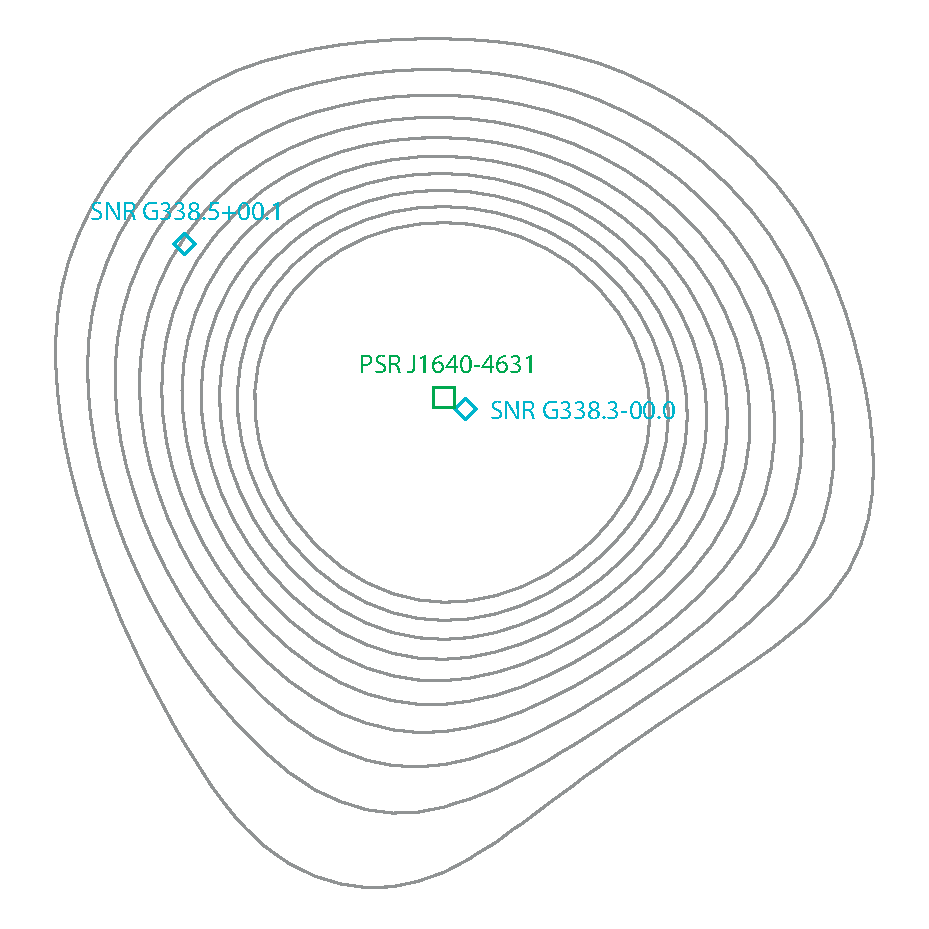
\includegraphics[width = \columnwidth]{figures/hess40}}
  \caption{Contour plot of HESS J1640-465 and surrounding objects of interest. Supernova remnants are shown as blue diamonds and pulsars as green squares}
  \label{fig:hess40}
\end{figure}

\paragraph{}
Possible sources for this gamma ray source. Kyle get your butt in here with that paper that answers this question. Yay, free research.

\section{Conclusions}
\paragraph{}
Bitch, we concluding now, making the statements that make a conclusion possible to be made with the words and the mouth. Bitch, we're flawless give us good grades.
\end{multicols}

\printbibliography[heading = bibintoc] % Include bibliography entry in ToC

\newpage

\appendix

\section{Derivation of galactic doppler shift}
\label{app:doppler}
\paragraph{}
Here we derive the equation found in Section~\ref{sec:gal-rot}. Looking at Fig.~\ref{fig:doppler}, we can (probably not) see the setup we're going to be dealing with here. In order to derive the velocity along the line of sight in the galactic plane, it is necessary to first consider the velocity field of the galactic plane. With coordinates centred on the GC, the velocity field can be expressed as
\begin{equation}
  \label{eq:vel-field}
  \mathbf{v}(x,y)=v(R)\cdot\!\left(\frac{y}{R},-\frac{x}{R}\right)\;,
\end{equation}
where \(x\), \(y\) are the Cartesian coordinates of point P, and \(R\) is the radial distance from point P to the GC, which by Pythagoras fulfils
\begin{equation}
  R^2=x^2+y^2\;.
\end{equation}

\begin{figure}[h]
  \centering
  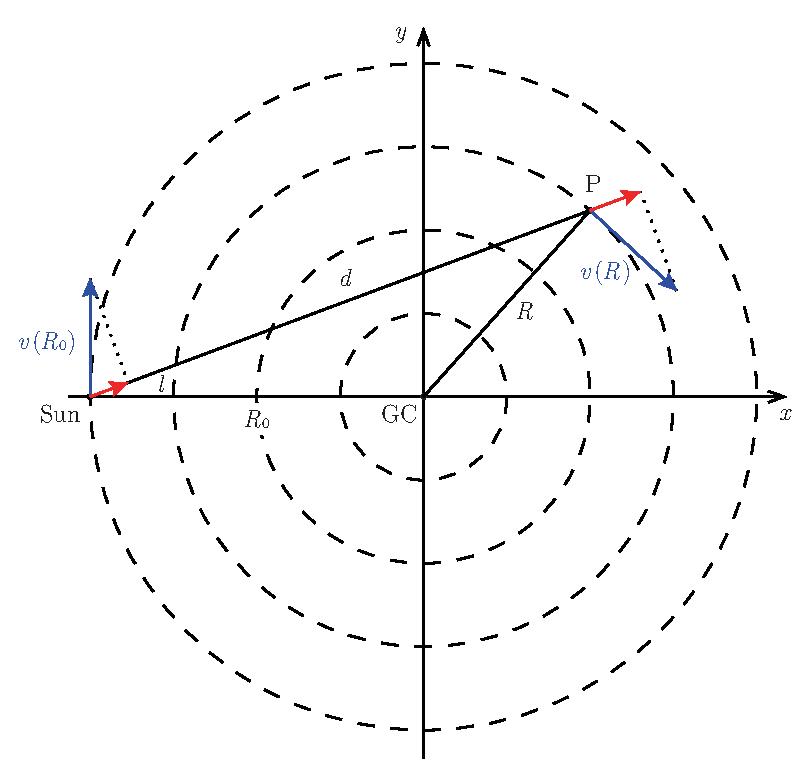
\includegraphics[width=13cm]{figures/doppler-shift}
  \caption{Velocity along line of sight in the galactic plane}
  \label{fig:doppler}
\end{figure}

In Eq.~\eqref{eq:vel-field}, \(v(R)\) is the radial velocity at point P with dependence on \(R\). This velocity field has galactic radial velocities pointing counter clockwise, which is what would be expected of a model for the Milky Way. In order to compute the component of velocities along the line of sight, it is worth considering first the dot product of the velocity field with the direction vector in the direction of the line of sight, \(\mathbf{\hat{d}}\):
\begin{align}
  \mathbf{v}(x,y)\cdot\mathbf{\hat{d}}&=v(R)\left[\left(\frac{y}{R},-\frac{x}{R}\right)\!\cdot(\cos{l},\sin{l})\right] \\
  &=v(R)\left(\frac{y\cos{l}-x\sin{l}}{R}\right) \\
  &=v(R)\left(\frac{y\cos{l}-x\sin{l}}{\sqrt{x^2+y^2}}\right)\;.
  \label{eq:vel-dot}
\end{align}
This expression gives the component of velocity in the \(\mathbf{\hat{d}}\) direction for any \((x,y)\). In order for this expression to be of any use in calculating the Doppler shift from the Mopra data, the coordinates need to be constained to the line of sight. The equation for the line of sight is given in vector form as:
\begin{equation}
  \lambda(d,l)=(d\cos{l}-R_0,d\sin{l})\;\,.
\end{equation}
Substituting the \(x\)- and \(y\)-coordinates from this expression in to Eq.~\eqref{eq:vel-dot} and expanding gives
\begin{equation}
  v_{los}(d)=\frac{v(R)R_0\sin{l}}{\sqrt{d^2-2R_0d\cos{l}+R_0^2}}\;\,.
\end{equation}
This expression only yields the absolute motion in the galaxy, and it is easy to see that for \(d=0\), \(v(0)=v(R)\sin{l}\) -- the sun's component of velocity along the line of sight. Subtracting this value gives us the equation used in the analysis of Mopra data:
\begin{equation}
  v_{los}(d)=\frac{v(R)R_0\sin{l}}{\sqrt{d^2-2R_0d\cos{l}+R_0^2}}-v(R_0)\sin{l}\;\,.
\end{equation}
In order to compute distances for a given velocity, the above equation can be rearranged to give
\begin{equation}
  d=R_0\left(\cos{l}\pm|\sin{l}|\sqrt{v_{rel}^2-1}\right)\;,
  \label{eq:d}
\end{equation}
where \(v_{rel}\) is `relative' velocity, given by
\begin{equation}
  v_{rel}=\frac{v(R)}{v_{los}+v(R_0)\sin{l}}\;\,.
\end{equation}

\section{Derivation of kinetic energy of expanding bubble}
\label{app:kinetic}
\paragraph{}
Here we derive the equation found in Section~\ref{sec:kinetic}. We begin with the familiar nonrelativistic equation for kinetic energy,
\begin{equation}
  \mathrm{KE} = \frac{1}{2} m v ^ 2 \, ,
\end{equation}
where \(m\) is the mass of the material displaced by the bubble (typically somewhat of an estimate) and \(v\) is the speed at which the bubble is expanding, i.e., the average speed of the gas in the reference frame of the object presumed to be at the centre. Mass \(m\) is given by mass density \(\rho\) multiplied by volume \(V\), and \(v\) can be found by halving the difference in speeds \(v_1\) and \(v_2\) of the front and back of the bubble:
\begin{equation}
  \mathrm{KE} = \frac{1}{2} \rho V { \left( \frac{\lvert v_1 - v_2 \rvert}{2} \right) }^2 \, .
\end{equation}
The volume \(V\) of the bubble is given by its radius, hence,
\begin{equation}
  \mathrm{KE} = \frac{1}{8} \rho \left( \frac{4}{3}\pi r^3 \right) {(v_1 - v_2)}^2
\end{equation} \begin{equation}
  \mathrm{KE} = \frac{1}{6} \pi \rho r^3 {(v_1 - v_2)}^2  \, .
\end{equation}
To find the radius of the bubble, we first determine the image slice which is halfway between the front and back slices of the bubble, ideally giving us a view of the bubble's cross section at the centre. Using Eq.~\ref{eq:d} outlined at the end of Appendix~\ref{app:doppler}, we can find the distance \(d\) to this slice. Now, consider a circle of radius \(d\) with its origin centred on the Solar System. This circle has a circumference of \(l = 2 \pi d\), and passes through all objects which are located a distance \(d\) away from us, including the middle of our chosen bubble. If we measure the angular width \(\Delta l\) of the bubble in degrees, then by a simple ratio the bubble has diameter \(\frac{\Delta l}{360}l\). Note this is diameter and not radius, so to get \(r\) we then halve this result. Thus,
\begin{equation}
  \mathrm{KE} = \frac{1}{6} \pi \rho {\left( \frac{1}{2} \frac{\Delta l}{360} 2 \pi d \right)}^3 {(v_1 - v_2)}^2  \, ,
\end{equation}
and we rearrange to get our final result:
\begin{equation}
  \mathrm{KE} = \frac{\pi ^ 4}{6} {\left( \frac{\Delta l}{360} \right)}^3 \rho d^3 {(v_1 - v_2)}^2 \, .
\end{equation}


\end{document}